\documentclass[12pt, unicode]{beamer}
\usetheme{Madrid}

\usepackage{luatexja}

\renewcommand{\kanjifamilydefault}{\gtdefault}

\title{自己紹介プレゼン}
\author{山本 竜也}
\institute[]{名古屋工業大学大学院\\工学専攻情報工学系プログラム}
\date{}

\begin{document}

\begin{frame}
  \maketitle
\end{frame}

\begin{frame}{もくじ}
  \begin{itemize}
    \item 自己紹介
    \item 課外活動団体の経験
    \item アルバイトの経験
    \item 研究内容
    \item 今後について
  \end{itemize}
\end{frame}

\begin{frame}{自己紹介}
  \begin{columns}
    \begin{column}{0.7\textwidth}
      \begin{block}{名前}
        \begin{itemize}
          \item 山本 竜也(やまもと たつや)
        \end{itemize}
      \end{block}

      \begin{block}{所属}
        \begin{itemize}
          \item 名古屋工業大学大学院 工学専攻\\情報工学系プログラム M1
        \end{itemize}
      \end{block}

      \begin{block}{趣味}
        \begin{itemize}
          \item YouTubeの動画鑑賞
          \item 将棋(将棋ウォーズ)
        \end{itemize}
      \end{block}
    \end{column}

    \begin{column}{0.25\textwidth}
      \begin{figure}[h]
        \centering
        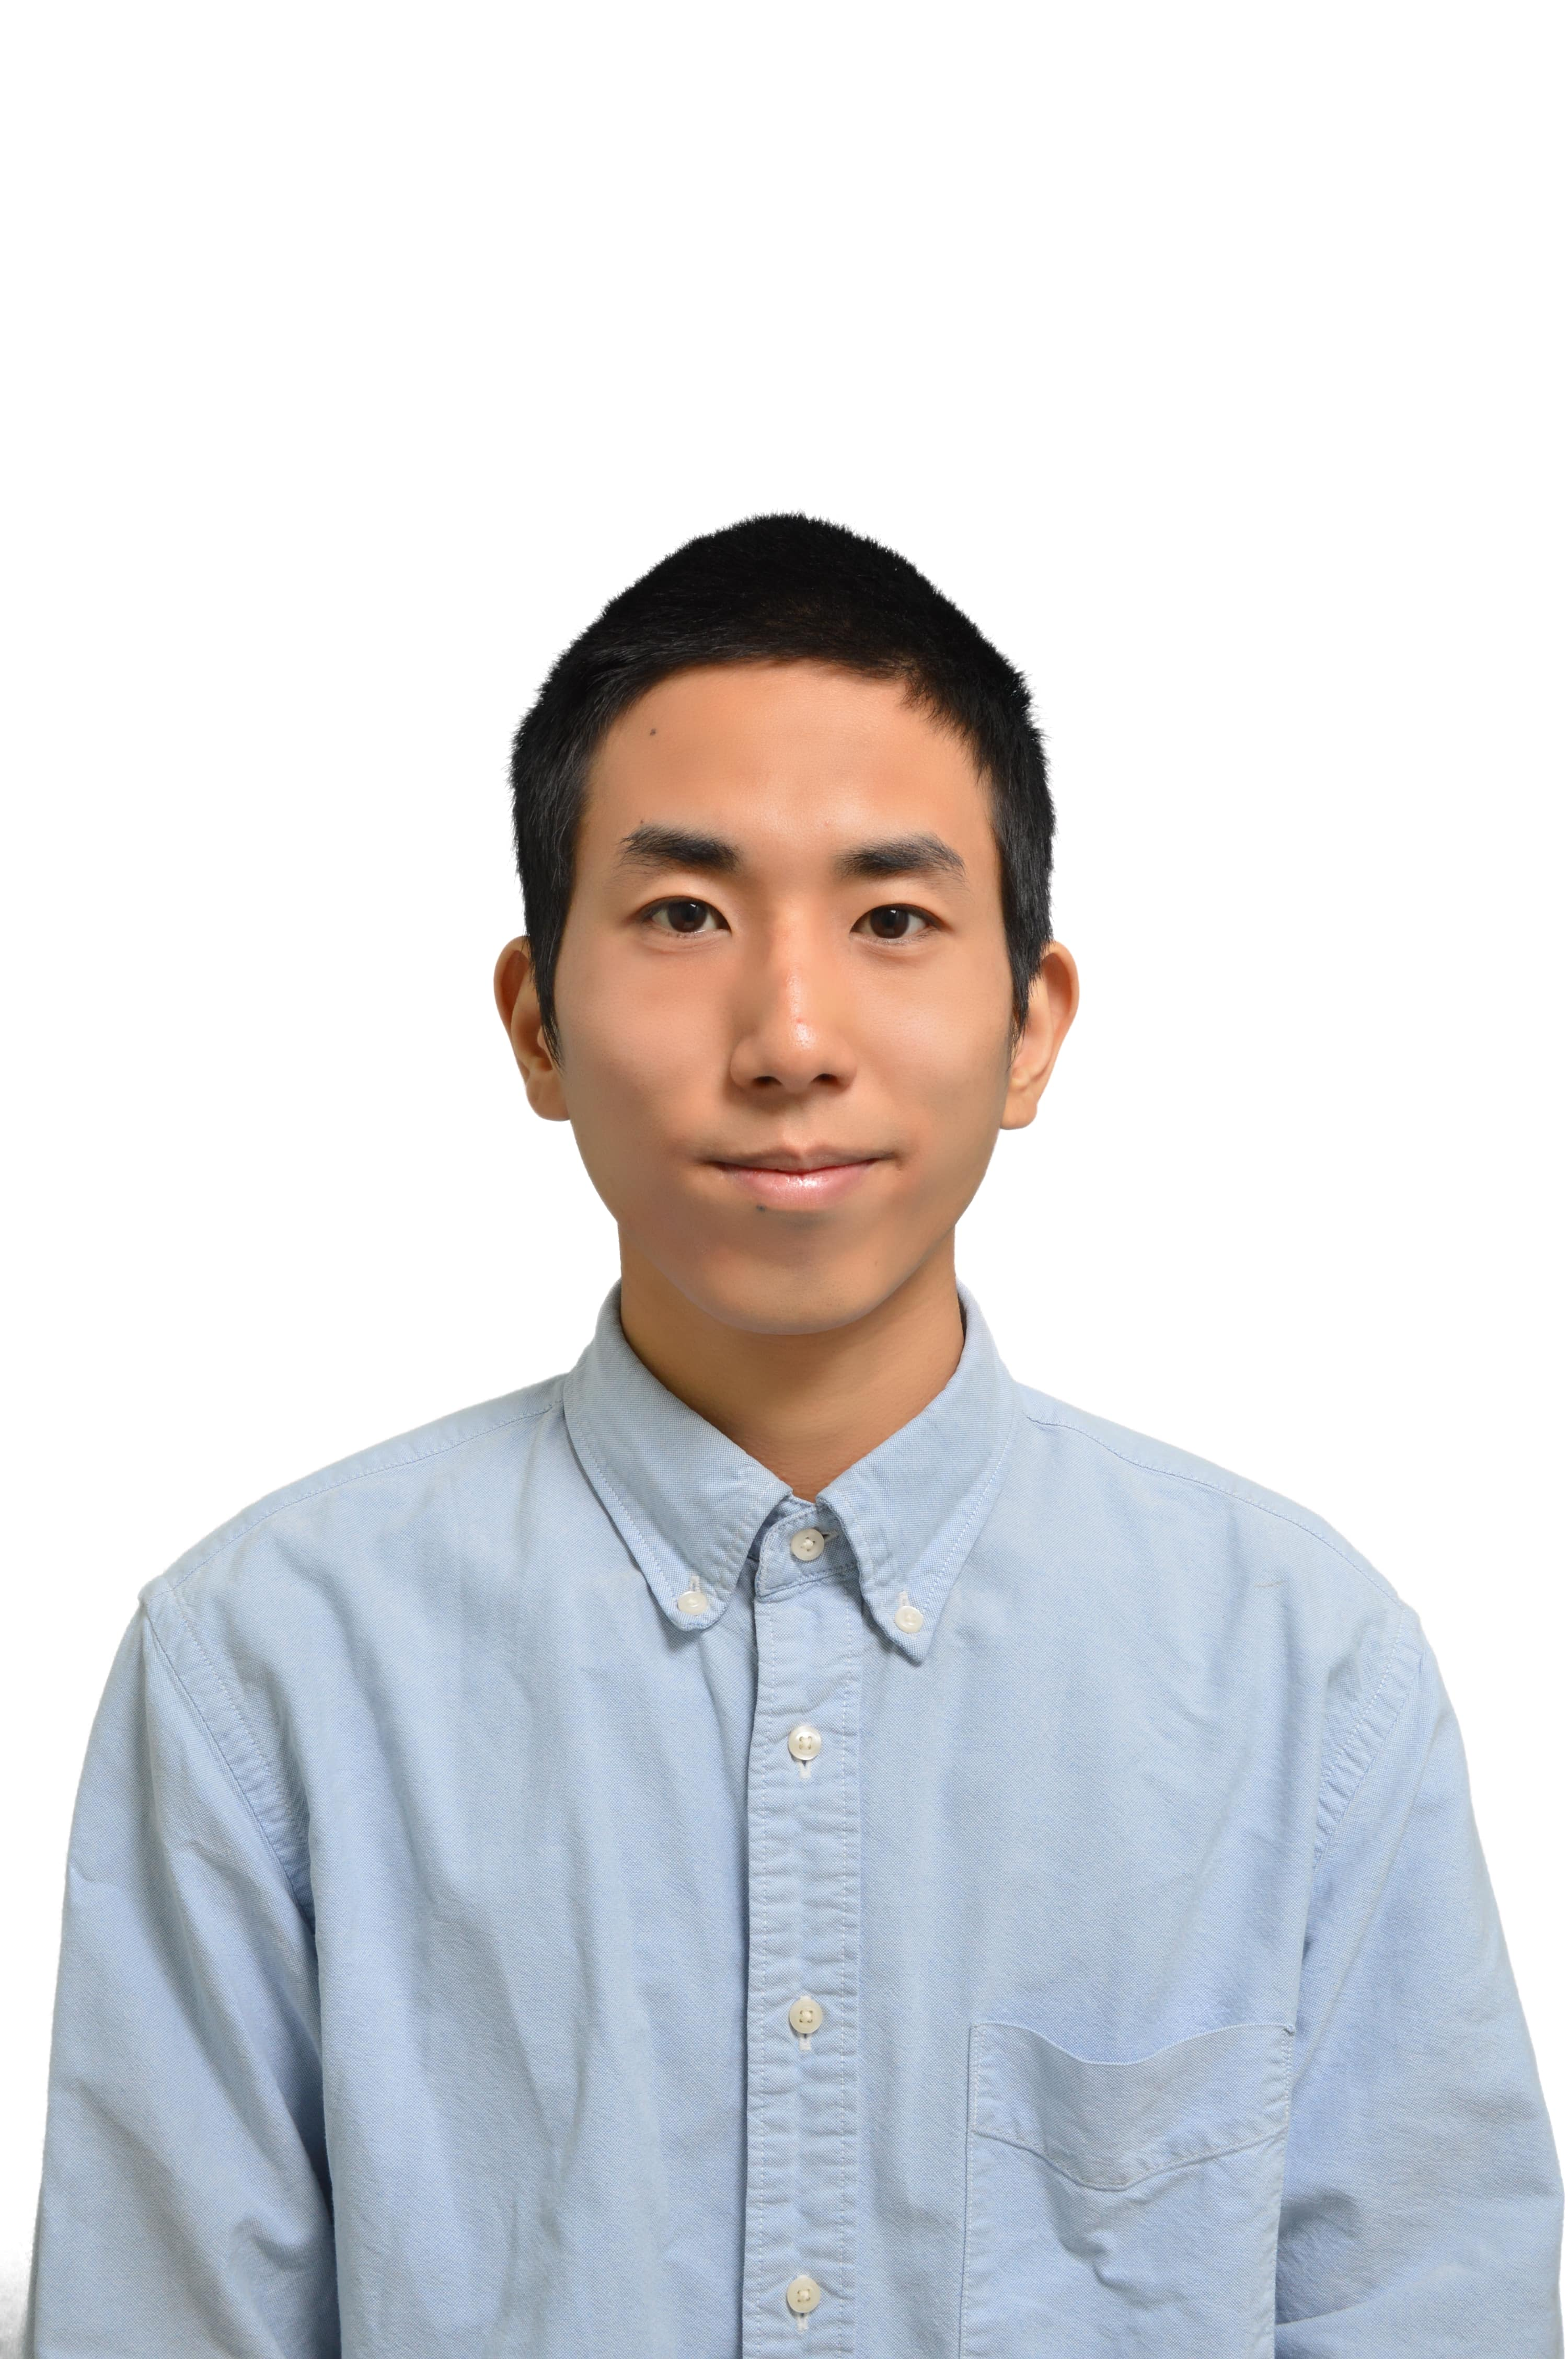
\includegraphics[width=\textwidth]{pictures/IDPhoto.jpg}
      \end{figure}
    \end{column}
  \end{columns}
\end{frame}

\begin{frame}{自己紹介}
  \begin{block}{受賞歴}
    \begin{itemize}
      \item 名古屋工業会賞
      \item 電子情報通信学会東海支部 令和三年度学業成績優秀賞
    \end{itemize}
  \end{block}

  \begin{figure}[h]
    \centering
    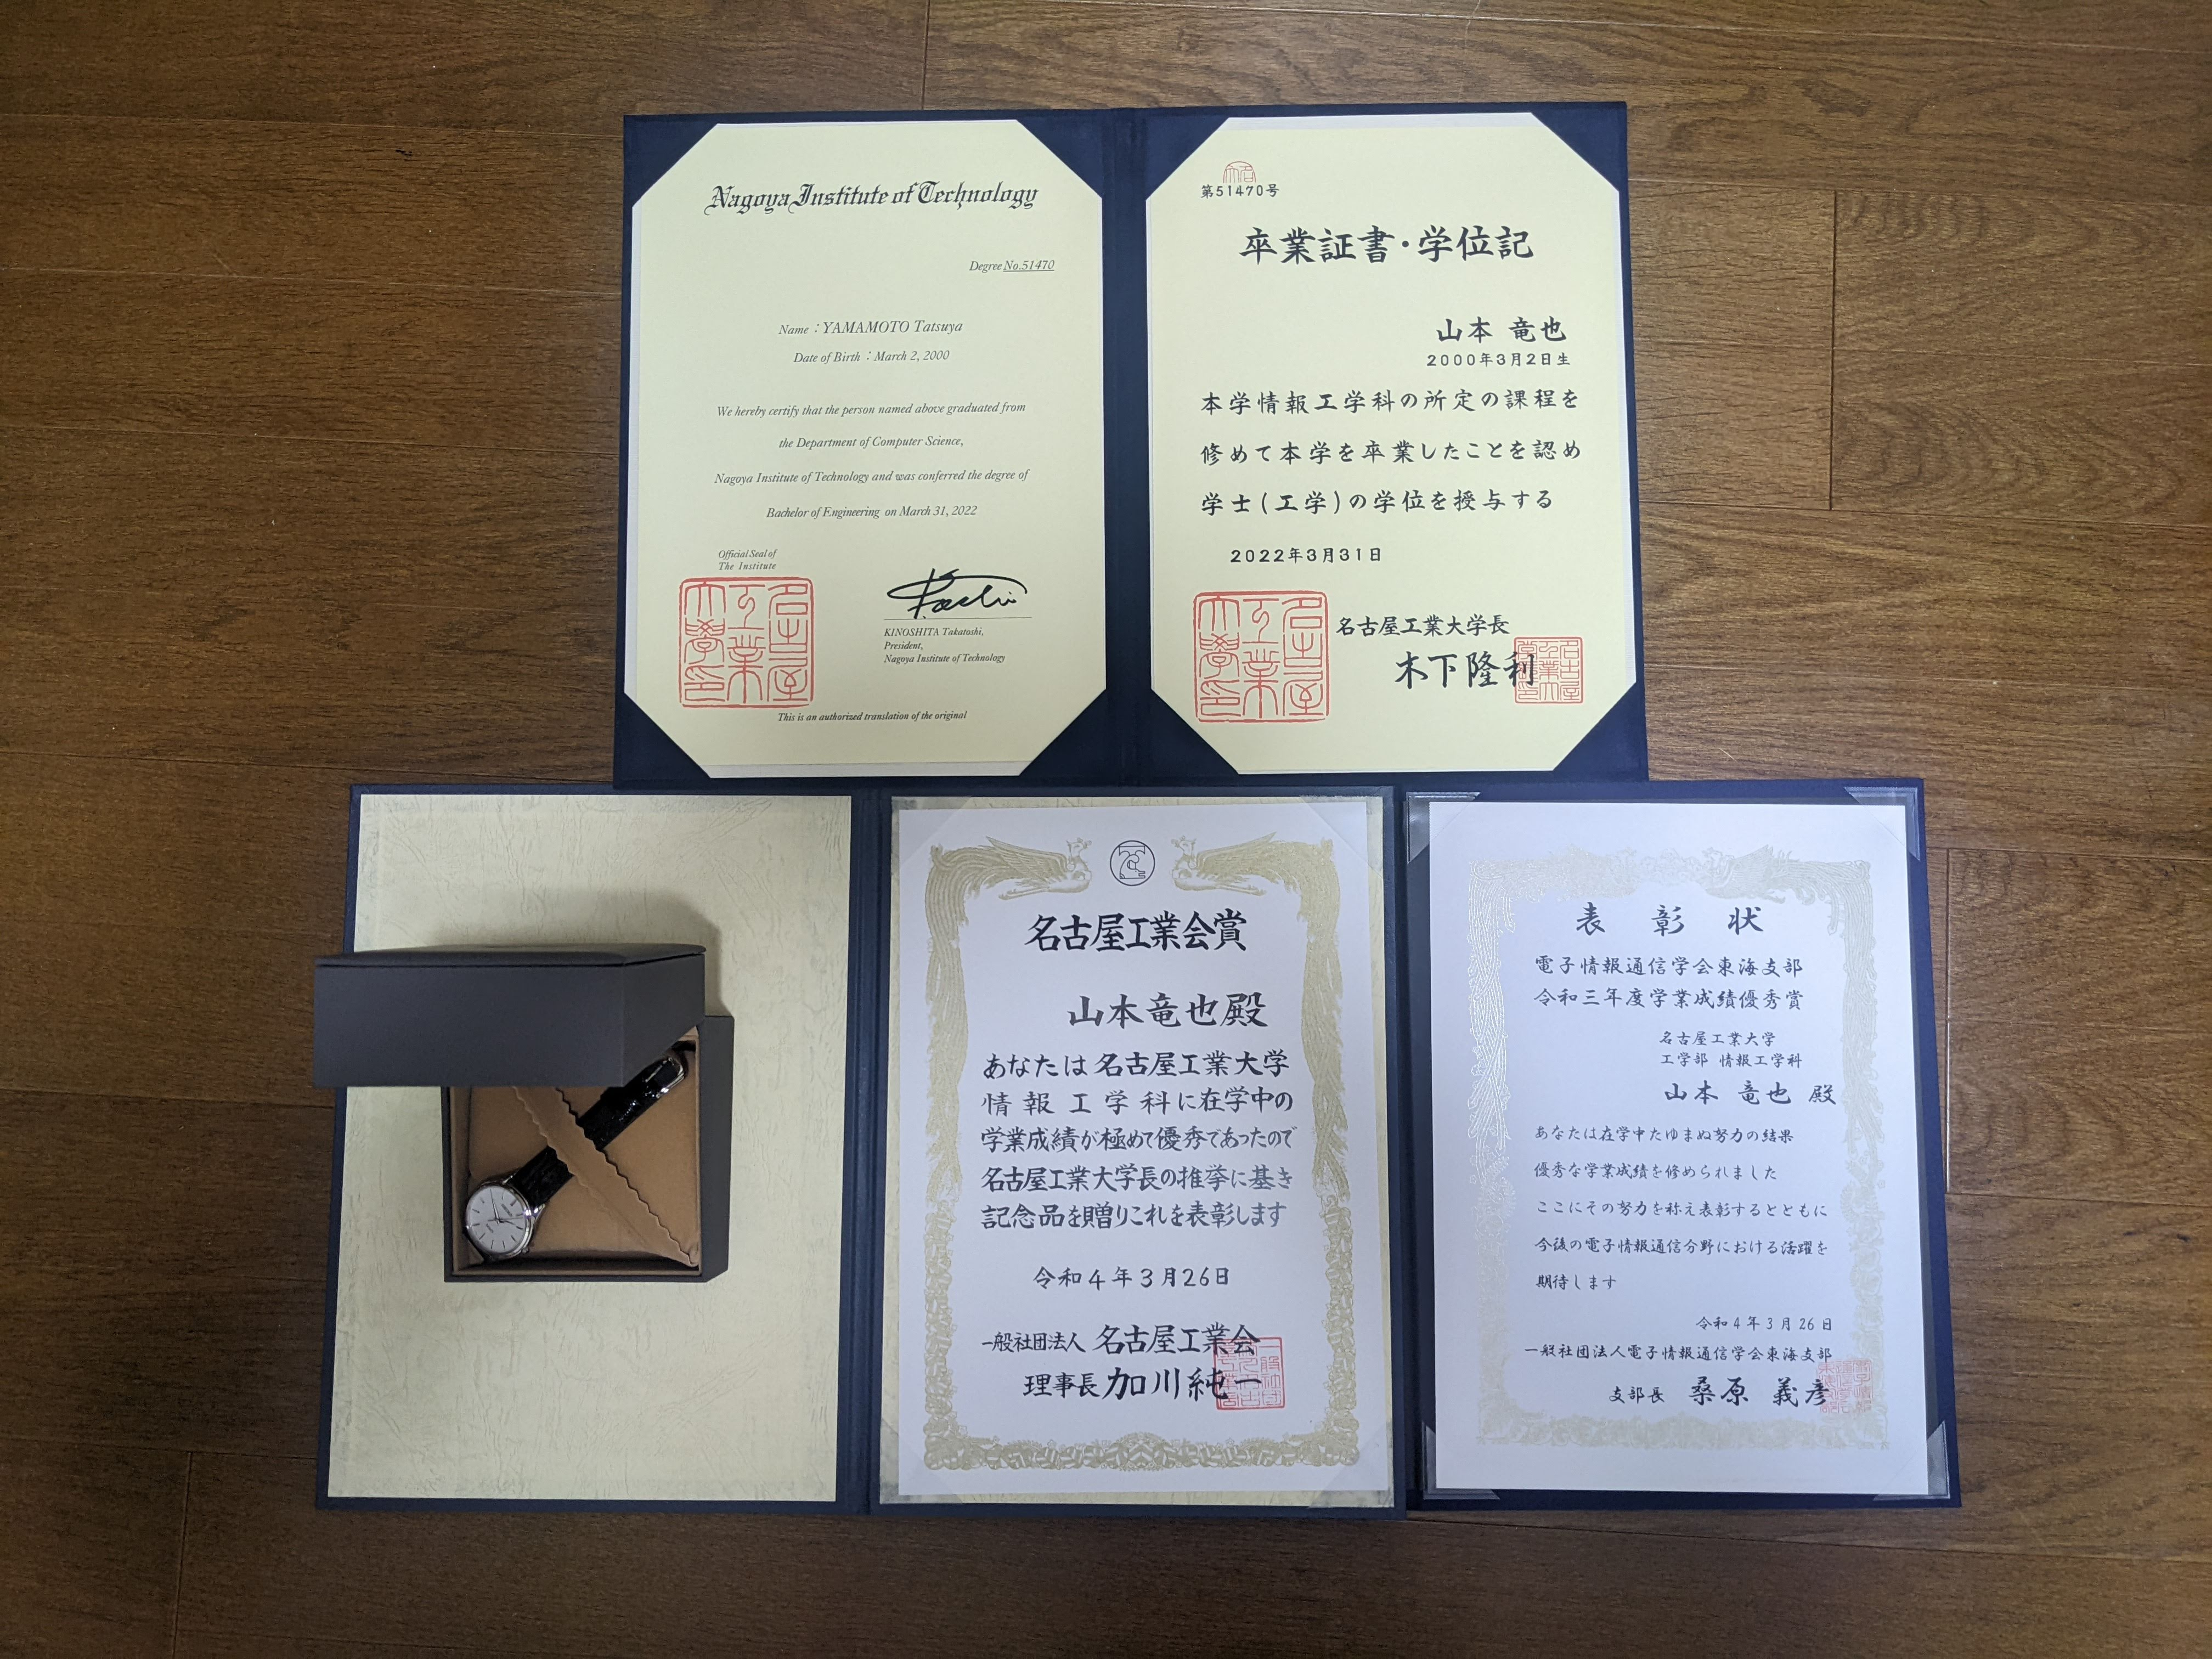
\includegraphics[width=0.6\textwidth]{pictures/Awards.jpg}
  \end{figure}
\end{frame}

\begin{frame}{課外活動団体の経験}
  \begin{columns}
    \begin{column}{0.8\textwidth}
      \begin{itemize}
        \item 名古屋工業大学公認課外活動団体C0de
        \item 一年生から三年生まで所属
        \begin{itemize}
          \item 二年生のときに庶務、三年生のときに部長
        \end{itemize}
      \end{itemize}
    \end{column}

    \begin{column}{0.2\textwidth}
      \begin{figure}[h]
        \centering
        
\includegraphics[width=0.9\textwidth]{pictures/C0de.png}
      \end{figure}
    \end{column}
  \end{columns}

  \begin{block}{やっていたこと}
    \begin{itemize}
      \item 先輩から引き継いだオンプレミスサーバの運用
      \begin{itemize}
        \item 運用していたサービスは公式HP, GitLab, NextCloud
        \item 引き継ぎをするのが難しかったため三年生のときに廃止
      \end{itemize}
      \item 新入部員向けのチュートリアル
      \begin{itemize}
        \item 同じ学年の仲間と一緒にスライドを作成して講義室で発表
        \item コロナの影響と運用コストが高かったため一年で中止
      \end{itemize}
    \end{itemize}
  \end{block}
\end{frame}

\begin{frame}{アルバイトの経験 一つ目}
  \begin{columns}
    \begin{column}{0.8\textwidth}
      \begin{itemize}
        \item 名古屋工業大学の情報基盤センター
        \item 2019年1月から現在まで継続
      \end{itemize}
    \end{column}

    \begin{column}{0.2\textwidth}
      \begin{figure}[h]
        \centering
        
\includegraphics[width=0.9\textwidth]{pictures/Pyrroline.png}
      \end{figure}
    \end{column}
  \end{columns}

  \begin{block}{やっていること}
    \begin{itemize}
      \item NITechピロリンという名古屋工業大学の学生向けアプリのサーバーサイドの開発
      \begin{itemize}
        \item iOS開発者, Android開発者との三人でのチーム開発
        \item 旧版のソースコードが古くて汚かったためリニューアル版をいちから開発
        \item 使用している主な技術はNode, TypeScript, MariaDB, NGINX, Docker, Git/GitHub, GitHub Actions, Swagger
      \end{itemize}
    \end{itemize}
  \end{block}
\end{frame}

\begin{frame}{アルバイトの経験 一つ目}
  \begin{columns}
    \begin{column}{0.3\textwidth}
      \begin{figure}[h]
        \centering
        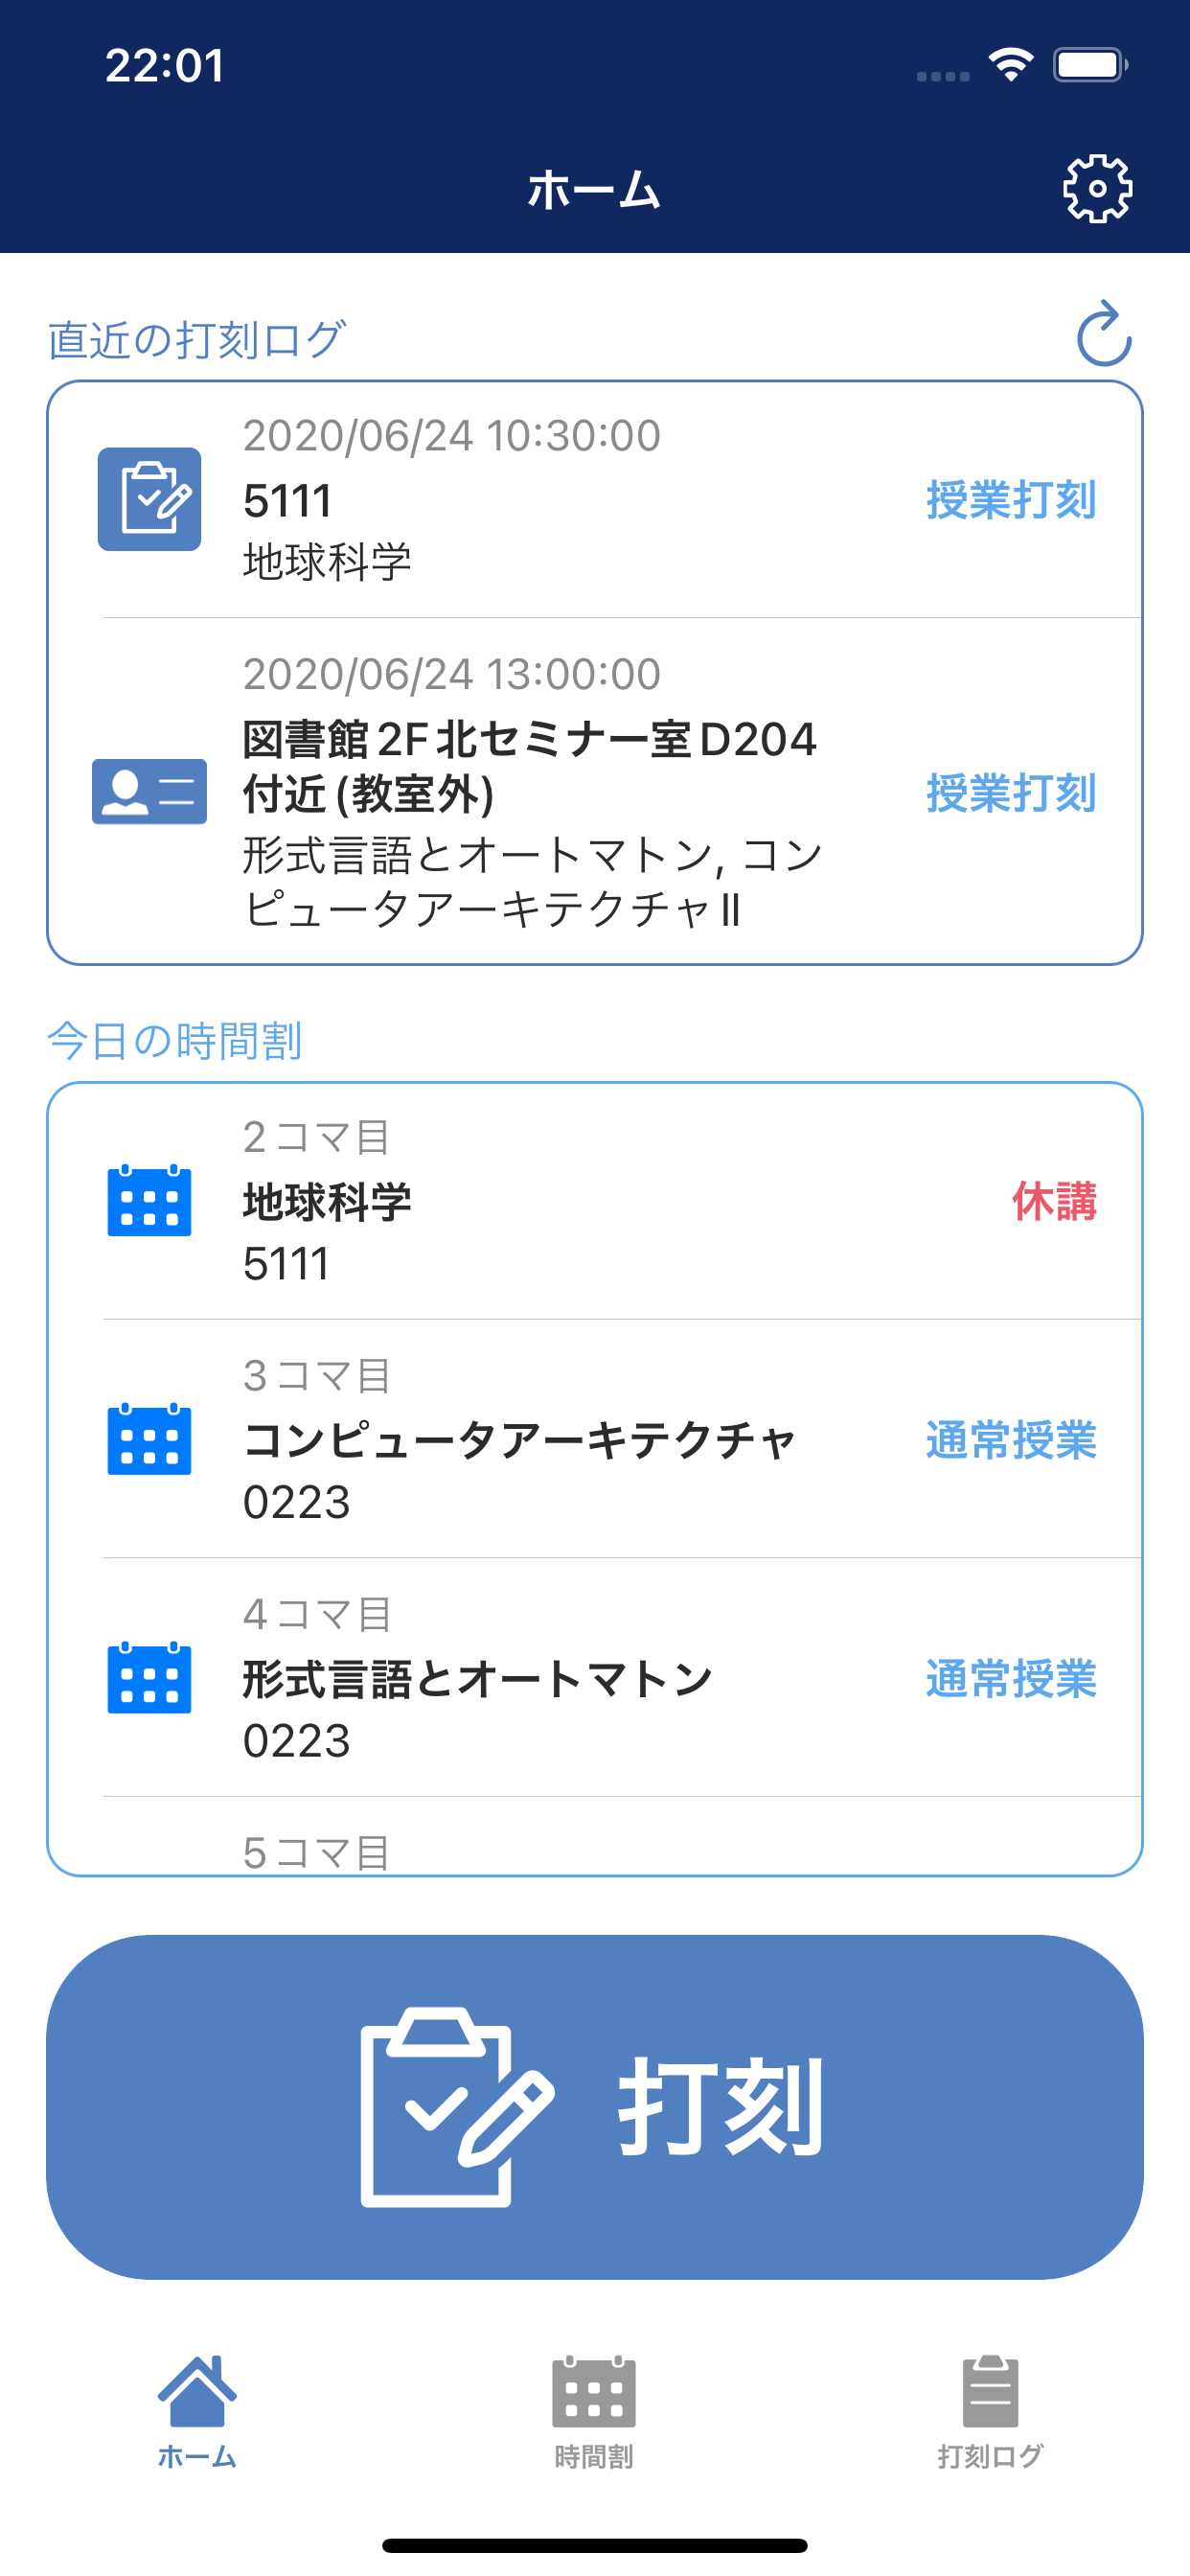
\includegraphics[width=0.9\textwidth]{pictures/PyrrolineHome.png}
      \end{figure}
    \end{column}

    \begin{column}{0.3\textwidth}
      \begin{figure}[h]
        \centering
        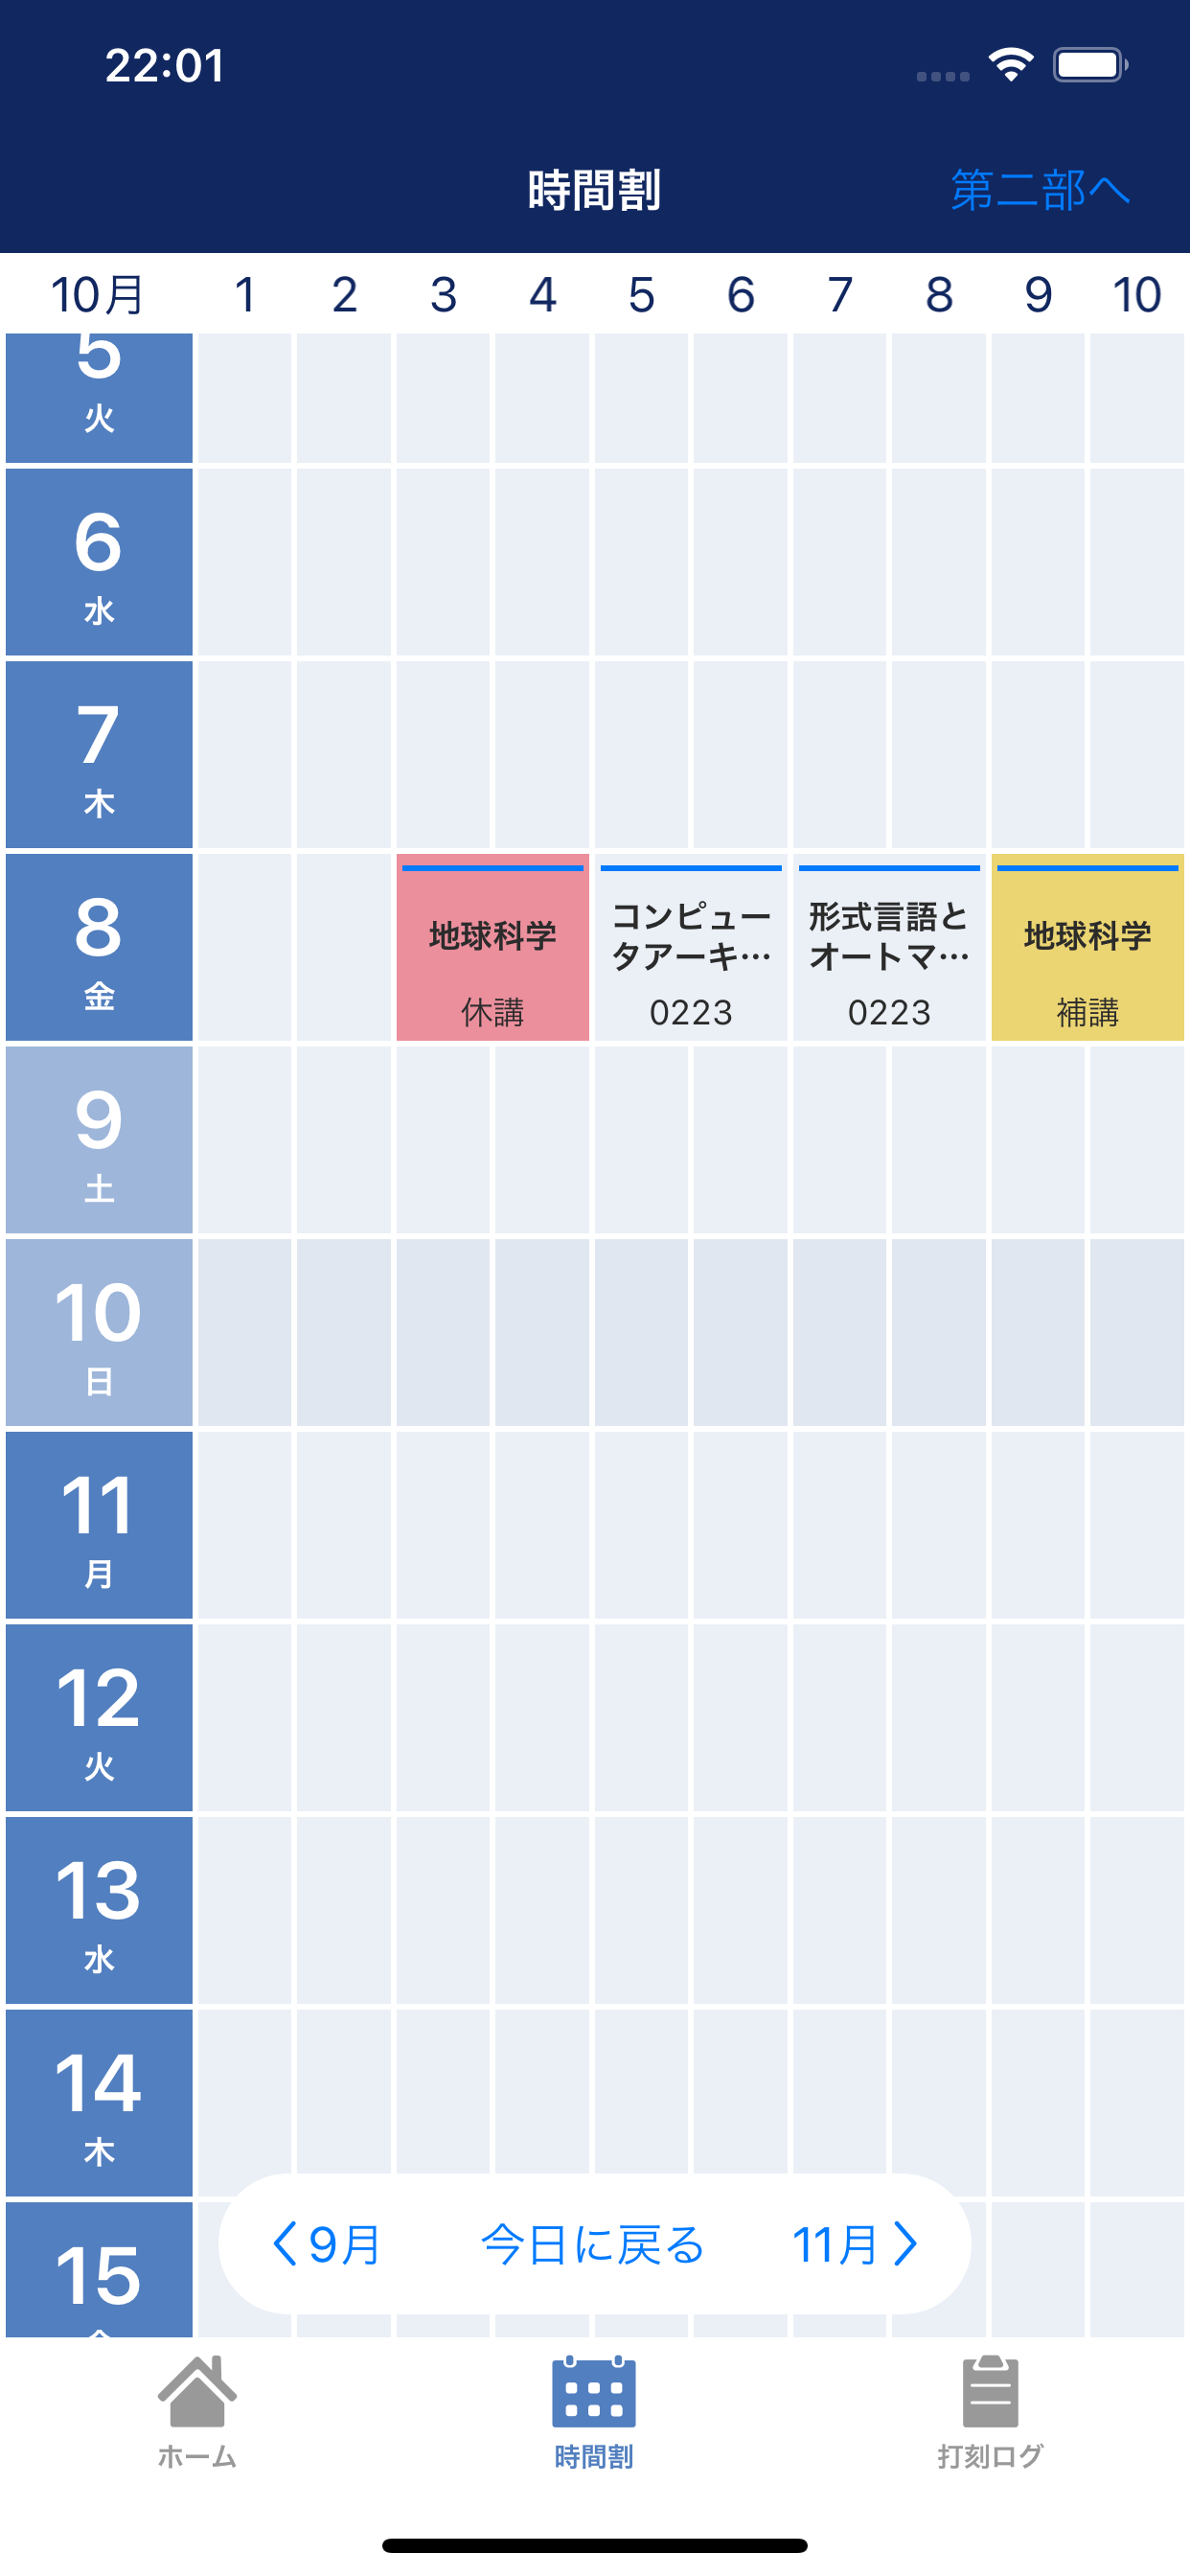
\includegraphics[width=0.9\textwidth]{pictures/PyrrolineLecture.png}
      \end{figure}
    \end{column}

    \begin{column}{0.3\textwidth}
      \begin{figure}[h]
        \centering
        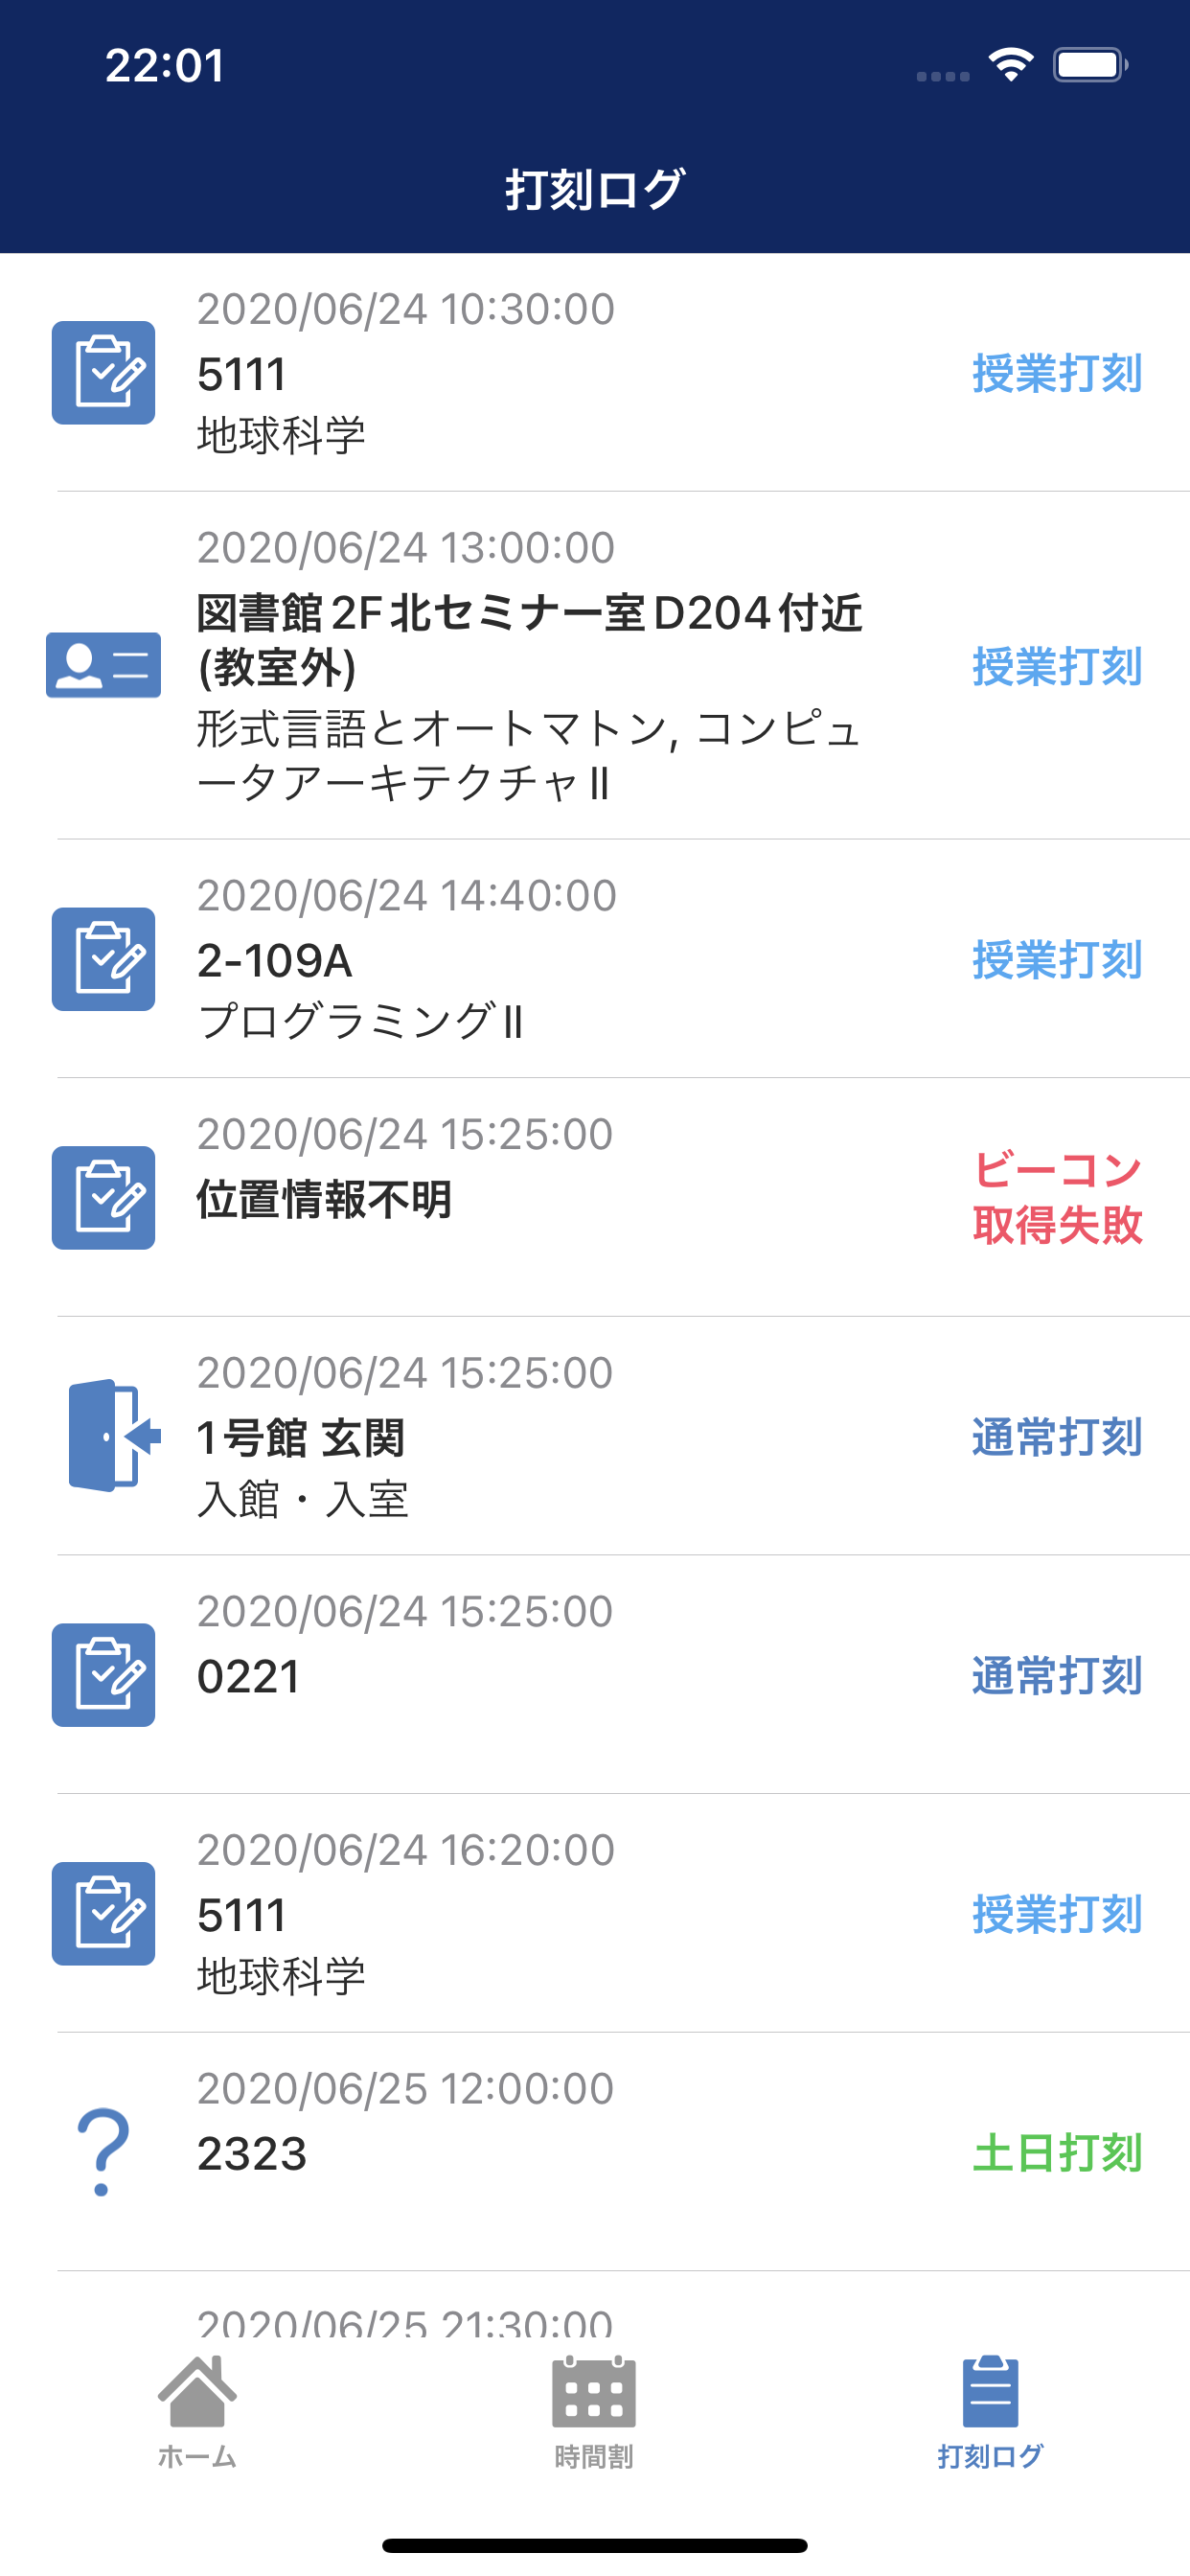
\includegraphics[width=0.9\textwidth]{pictures/PyrrolineStamp.png}
      \end{figure}
    \end{column}
  \end{columns}
\end{frame}

\begin{frame}{アルバイトの経験 二つ目}
  \begin{columns}
    \begin{column}{0.8\textwidth}
      \begin{itemize}
        \item ツーエス・テクノロジーズ株式会社
        \begin{itemize}
          \item 名古屋に本社を持つベンチャー企業
        \end{itemize}
        \item 2019年2月から現在まで継続
      \end{itemize}
    \end{column}

    \begin{column}{0.2\textwidth}
      \begin{figure}[h]
        \centering
        
\includegraphics[width=0.9\textwidth]{pictures/2ST.png}
      \end{figure}
    \end{column}
  \end{columns}

  \begin{block}{やっていたこと/やっていること}
    \begin{itemize}
      \item Webアプリのテストやバグ取り
      \item WebアプリやAPIサーバのDocker化
      \item Visual Basicで書かれたプログラムのJavaへの変換
      \begin{itemize}
        \item 使用したことのある主な技術はAngular, Node, TypeScript, MongoDB, NGINX, MQTT, Docker, Git/GitHub
      \end{itemize}
    \end{itemize}
  \end{block}
\end{frame}

\begin{frame}{研究内容}
  \begin{itemize}
    \item DPDKの送受信スレッドでアプリケーションを実行する\\新たな分散処理フレームワークを提案
    \begin{itemize}
      \item DPDKによるL2通信を用いる
      \begin{itemize}
        \item TCP/IPのオーバーヘッドをなくすことができる
        \item 高速なパケットI/Oを用いることができる
      \end{itemize}
      \item DPDKの送受信スレッドでアプリケーションを実行する
      \begin{itemize}
        \item CPUリソースを有効に活用することができる
        \item CPUのキャッシュ内で演算することができる
      \end{itemize}
    \end{itemize}
  \end{itemize}

  \begin{figure}[h]
    \centering
    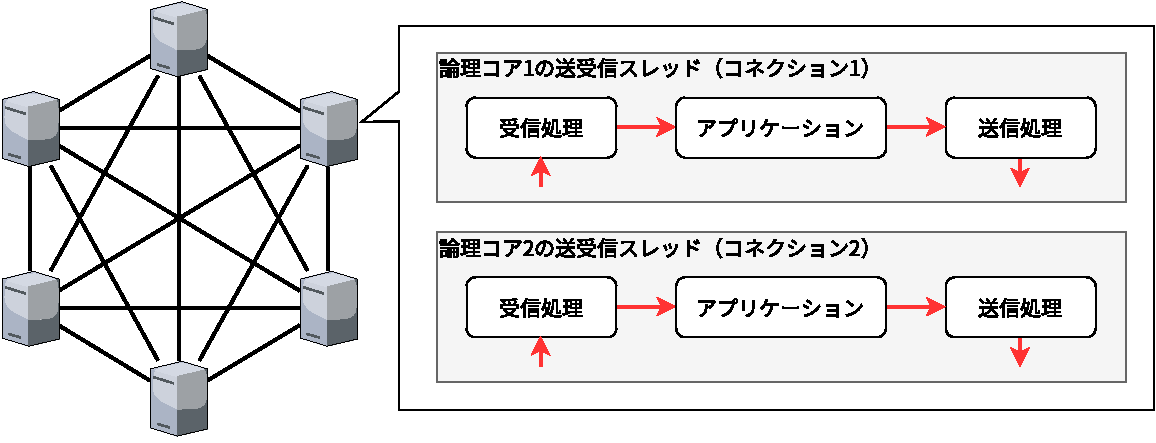
\includegraphics[width=0.9\textwidth]{pictures/Research.pdf}
  \end{figure}
\end{frame}

\begin{frame}{今後について}
  \begin{block}{目指しているエンジニア像}
    \begin{itemize}
      \item 人に使ってもらえるプロダクトを作るエンジニア
      \begin{itemize}
        \item 大学に入って本格的にプログラミングを始めた頃はプログラミング言語に興味があった
        \item C0deやNITechピロリンの経験を通して、自分たちが作った\\アプリをユーザが使ってくれるのは嬉しいと思うようになった
      \end{itemize}
    \end{itemize}
  \end{block}

  \begin{block}{企業選びの軸}
    \begin{itemize}
      \item コミュニケーションが活発な会社
      \begin{itemize}
        \item チーム開発ではメンバー間で議論することが大切ということをNITechピロリンの開発で実感
      \end{itemize}
      \item 使用する技術についてのこだわりはあまりない
    \end{itemize}
  \end{block}
\end{frame}

\begin{frame}{質問}
  \begin{block}{エンジニアの方にお答えいただきたいもの}
    \begin{itemize}
      \item 社内のコミュニケーションはどんな形で行われていますか
      \item 今の会社に入社することにした決め手は何でしたか
      \item 新入社員だったときの業務内容はどんな感じでしたか
    \end{itemize}
  \end{block}

  \begin{block}{人事の方にお答えいただきたいもの}
    \begin{itemize}
      \item 新卒の採用にあたって重視していることは何ですか
    \end{itemize}
  \end{block}
\end{frame}

\end{document}
